In this section, we compare novel SAF-based methods with a
variety of (social) collaborative filtering baselines:
\begin{enumerate}
\item {\bf Most Likely Class Constant Predictor (Const)}
\item {\bf Nearest Neighbor (NN)}~\cite{bellkor}
\item {\bf Matrix Factorization (MF)}~\cite{pmf}
\item {\bf Social Matchbox (SMB)}~\cite{Noel2012NOF}
\end{enumerate}
Here, Const serves as a lower bound on performance, NN and MF are two
well-known state-of-the-art \emph{non-social} collaborative filtering
algorithms, and SMB is a state-of-the-art \emph{social} collaborative
filtering algorithm employing matrix factorization with social
regularisation.

Among the novel SAF methods, we analyse four different sets of 
social affinity features:
\begin{enumerate}
\item {\bf Interaction Social Affinity Features (ISAF)}
\item {\bf Activity-based Social Affinity Features (ASAF)} for 
  \begin{enumerate}
  \item {\bf Group Memberships}
  \item {\bf Page Likes}
  \item {\bf Favourites}
  \end{enumerate}
\end{enumerate}
Furthermore, for these four classes of features, we train
one of three classifier types, leading to the following
classes of SAF recommenders evaluated in our experiments:
\begin{enumerate}
  \item {\bf Na\"{i}ve Bayes (NB-ISAF, NB-ASAF)}
  \item {\bf Support Vector Machines (SVM-ISAF, SVM-ASAF)}
  \item {\bf Logistic Regression (LR-ISAF, LR-ASAF)}
\end{enumerate}
NB uses a standard Na\"{i}ve Bayes implementation, 
SVM and LR are both implemented using \textit{LIBLINEAR}~\cite{liblinear}.

In all experiments, we report average classification accuracy
(fraction of correct classifications in held-out test data) using
10-fold cross validation and provide standard error bars corresponding
to 95\% confidence intervals.
%#suvash#
%Accuracy is defined as  
%\begin{align*}
%accuracy = \frac{\#\ correct\ predictions}{\#\ predictions}
%\end{align*}

Fig~\ref{Fig1} compares the above baselines and SAF algorithms.  In
all of these experiments, SAF variants performed statistically
significantly better than the best baseline (SMB), except for NB-ASAF
which we conjecture is due to violation of feature independence
assumptions that become more pronounced as the number of features
increases (n.b., NB-ISAF uses 22 features while NB-ASAF uses 1000's of
features).

%%%%%%%%%%%%%%%%%%%%%%%%%%%%%%%%%%%%%%%%%%%%%%%%%%%%%%%%%%%%%%%%%%%%%%%%%%%
\begin{figure*}[tbh!]
%\centering
\hspace{-6mm}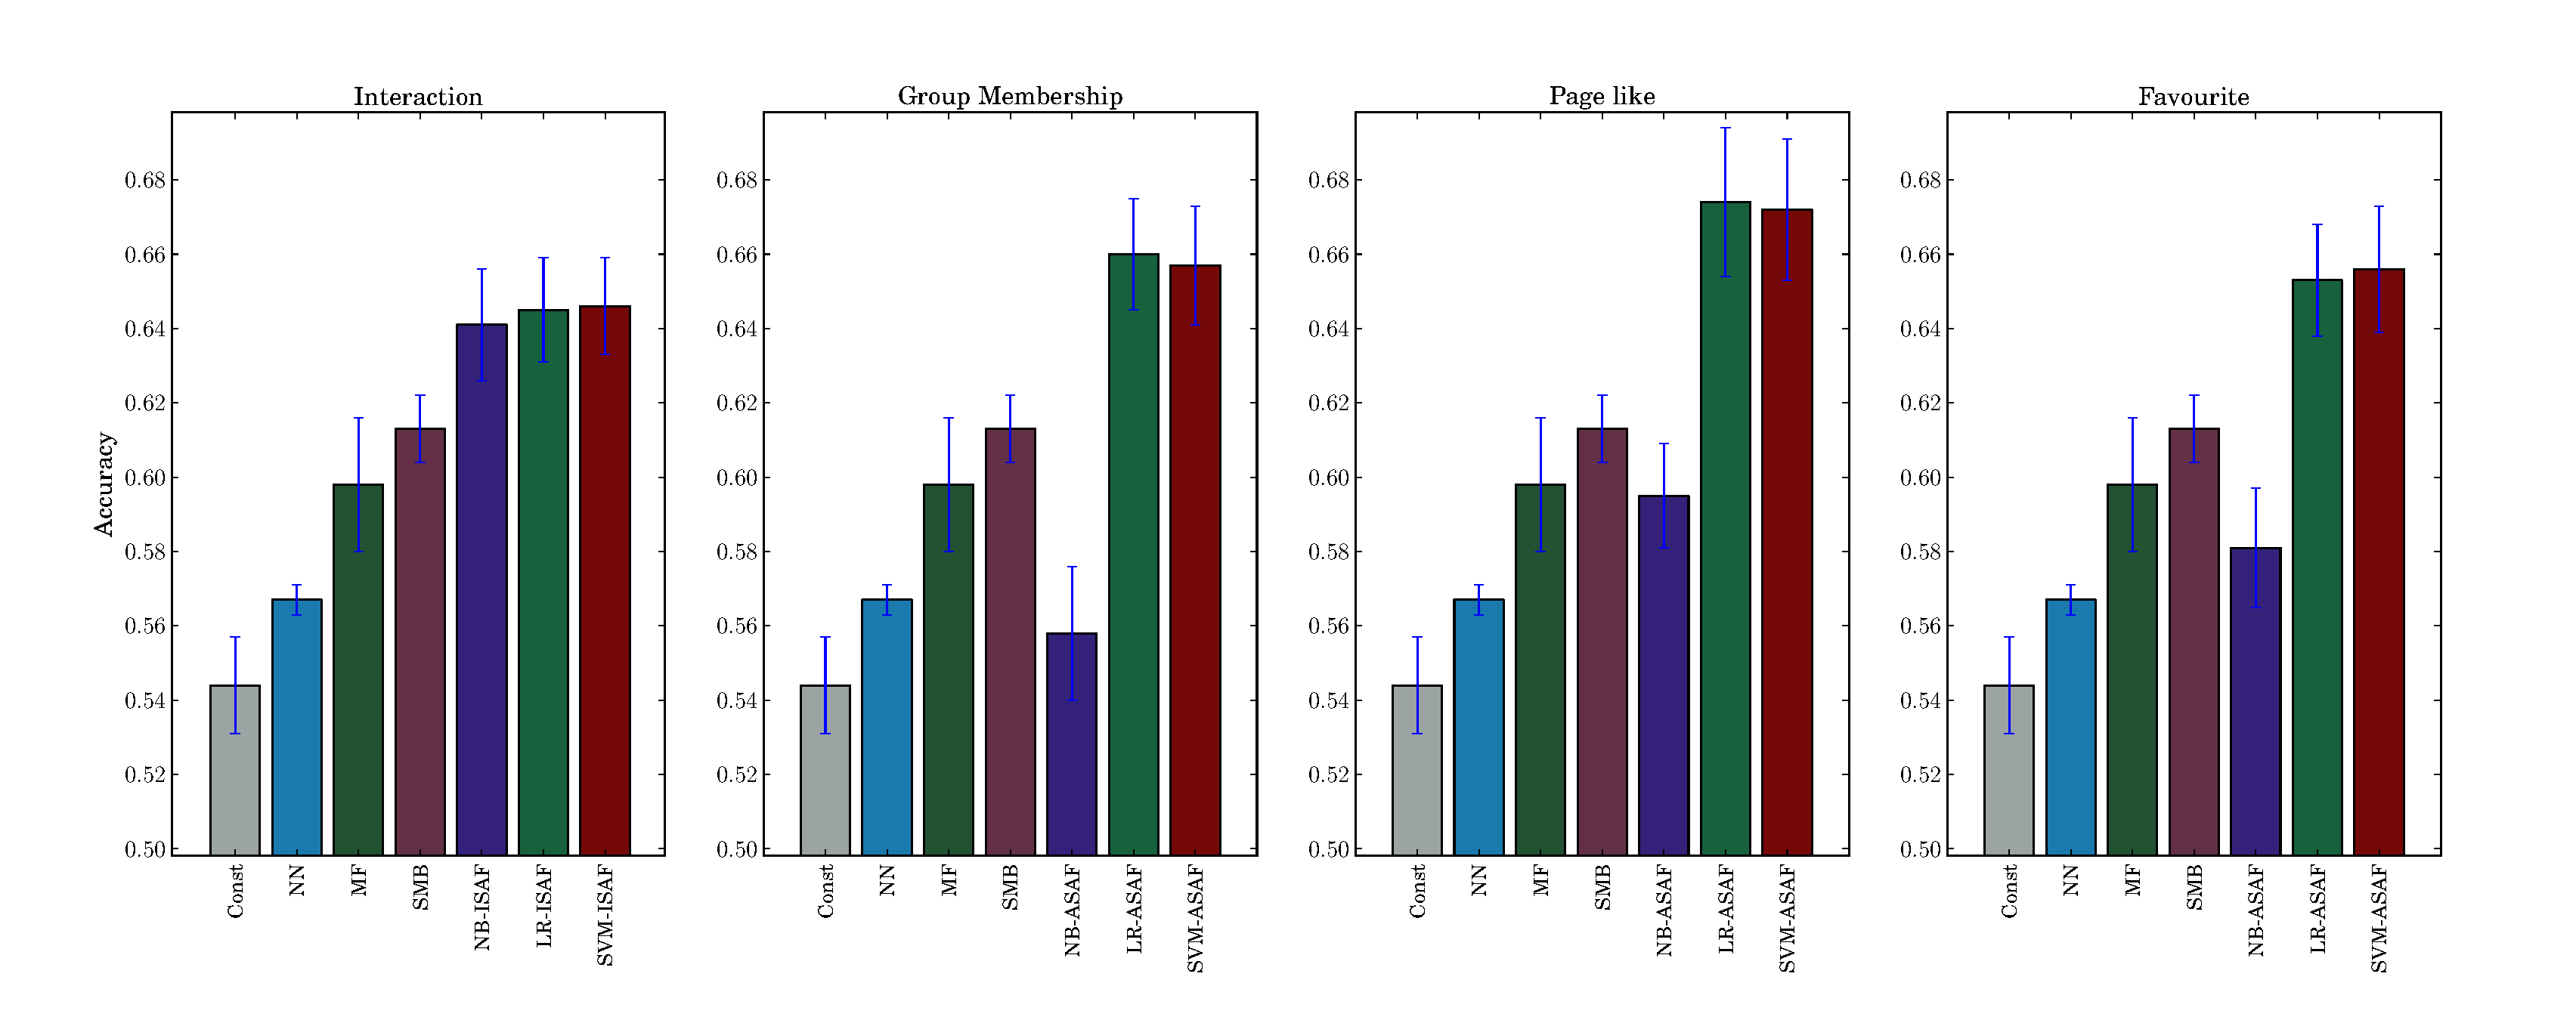
\includegraphics[height=80mm,width=190mm]{data/newPlots/accuracy.eps}
\vspace{-6mm}
\caption{Comparision of a simple baseline (Const), two collaborative
  filtering baselines (NN and MF), a social collaborative filtering
  baseline (SMB) and novel SAF recommenders using different feature
  sets (one ISAF and three ASAF sets) and classifiers (NB,LR,SVM).
  The best SAF-based model (LR-ASAF) --- for Page likes --- significantly outperforms
  all baselines by at least 6\%.  Combining all four feature sets (not shown)
  does not lead to improvement over Page likes features alone.}
\label{Fig1}
\end{figure*}
%%%%%%%%%%%%%%%%%%%%%%%%%%%%%%%%%%%%%%%%%%%%%%%%%%%%%%%%%%%%%%%%%%%%%%%%%%%

%%%%%%%%%%%%%%%%%%%%%%%%%%%%%%%%%%%%%%%%%%%%%%%%%%%%%%%%%%%%%%%%%%%%%%%%%
\begin{figure*}[tbh!]
\centering
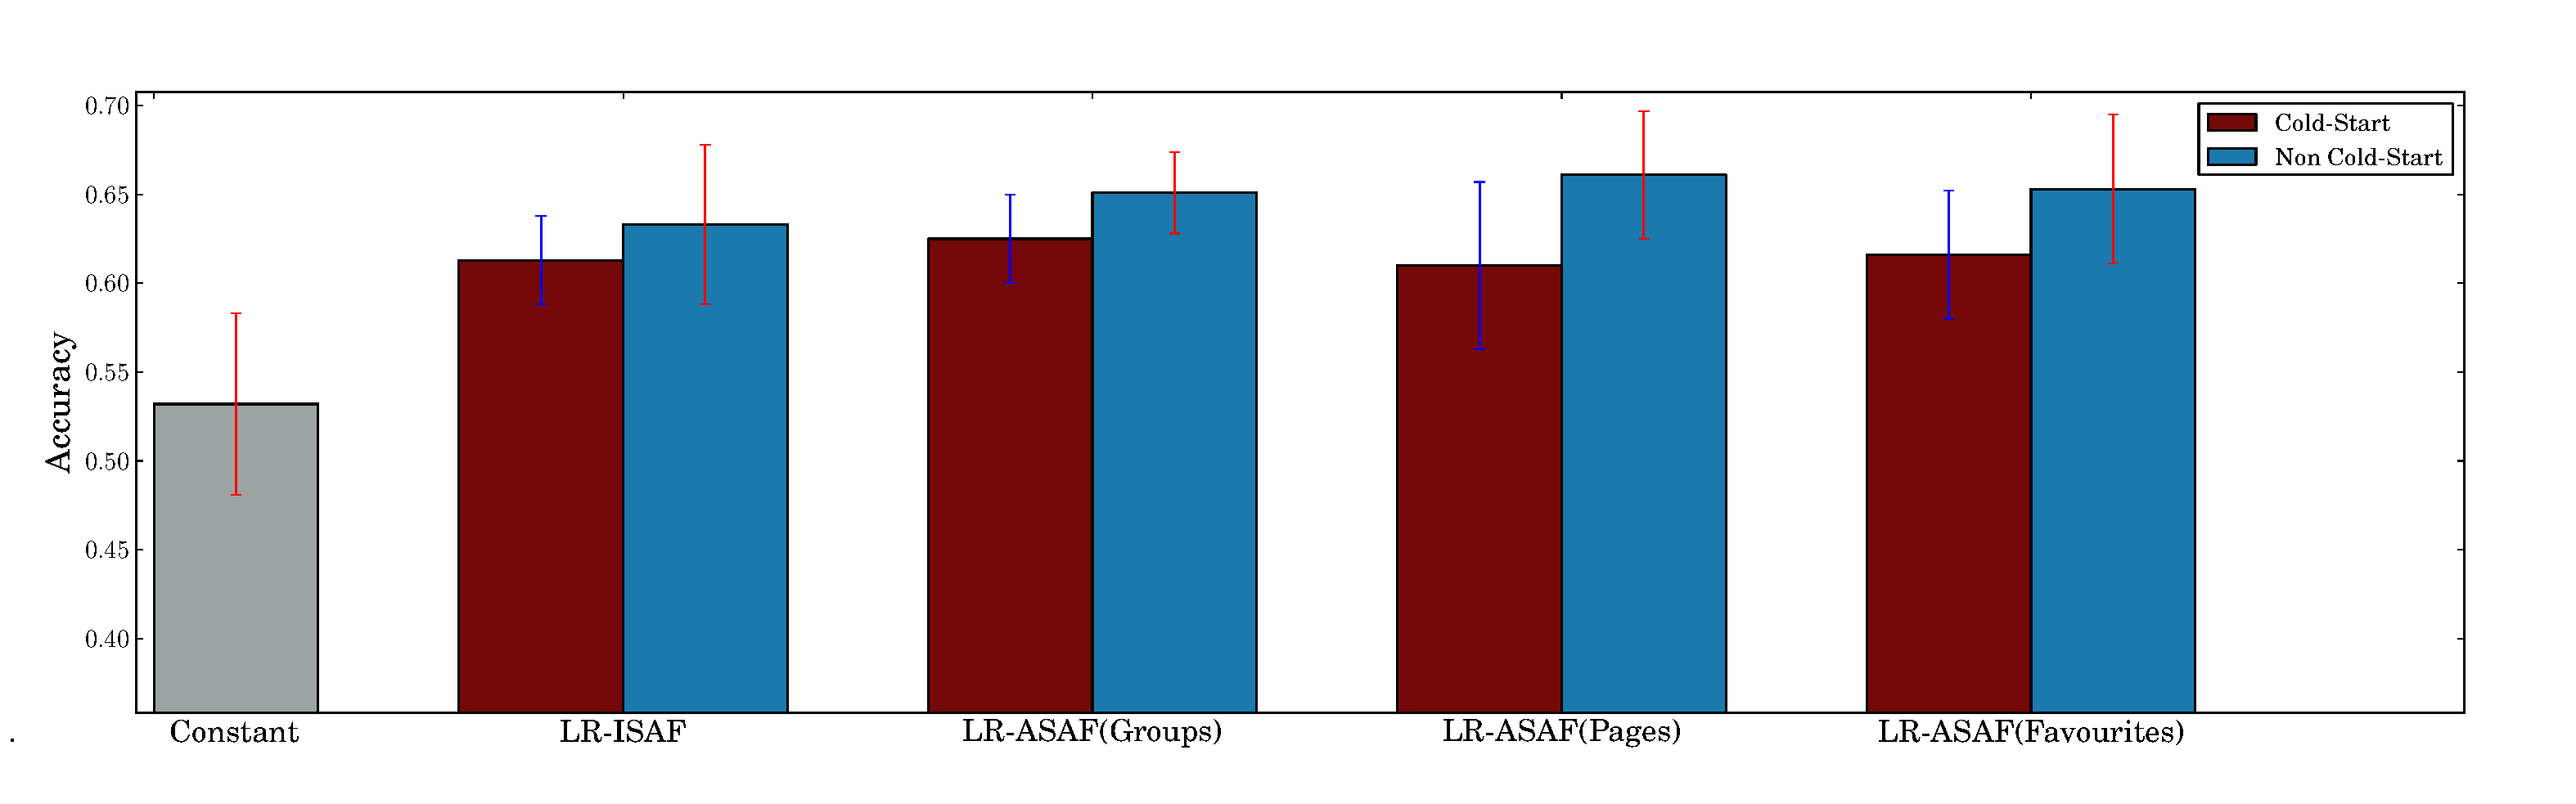
\includegraphics[width=180mm,height=50mm]{data/newPlots/cold_start.eps}
\vspace{-6mm}
\caption{Cold-start evaluation of SAF: accuracy evaluated on cold-start users 
  outperforms the most likely class (Constant) predictor baseline and is
  somewhat comparable to the non cold-start case when all test user data is \emph{not}
  withheld from training.}
\label{fig:coldstart}
\end{figure*}
%%%%%%%%%%%%%%%%%%%%%%%%%%%%%%%%%%%%%%%%%%%%%%%%%%%%%%%%%%%%%%%%%%%%%%%%%
 

In terms of the best recommenders, we observe that LR-ASAF and
SVM-ASAF perform comparably to each other and learn quite well despite
the large size of this ASAF feature set.  Overall, \emph{LR-ASAF
  performs 6\% better than the best baseline for page likes}.  We
combined all four features sets in a fifth experiment (not shown) and
remark that none of NB, LR, or SVM with all features outperformed
LR-ASAF with just page likes.  We also note that all ISAF variants
statistically significantly outperform all (social) collaborative
filtering baselines.  Hence, w.r.t.\ this Facebook dataset, we
conclude that (a) \emph{SAF with any available feature set} is sufficient
to outperform existing (social) collaborative filtering baselines and
that (b) if one wanted to minimise the permissions an App requests
then it seems \emph{SAF with page likes} alone is sufficient to
outperform all other feature sets (alone or combined).

It is important to consider why ASAFs outperform ISAFs.  We conjecture
the reasons for this are quite simple: ISAFs can only see the
\emph{friends} of user $u$ whereas ASAFs are able to look at all
users, independent of $u$'s friends.  Hence, given the relative
sparsity of friend-only data in Facebook compared to the greater
Facebook population (at least the subset of the population the App
collected) and also the relative number of ISAFs compared to ASAFs,
ASAFs appear to draw on a much larger set of SAGs that in turn draw on
a much larger user population.  Among ASAFs, page likes are the most
predictive followed by group membership and favourites.  This
reinforces our conjecture that data sparsity can hurt SAF since we
note from Table~\ref{tab:interests} that page likes are more prevalent
than groups and favourites.

Comparing SAF to the state-of-the-art in social collaborative
filtering as represented by Social Matchbox (SMB)~\cite{Noel2012NOF},
we observe that SAF consistently outperforms it.  We note that the key
difference of SAF vs. SMB is that SAF exploits the predictiveness of
fine-grained interactions and activities, whereas most
%#suvash#
social collaborative filtering
approaches~\cite{socinf,rrmf,ste,sorec,sr,Noel2012NOF,lla} instead
collapse the diverse set of interactions into a single aggregate
statistic for each pair of users.  The performance of SAF-based
recommenders suggests that the aggregation of all social information
into aggregate statistics (without learning which interactions or
activities are most informative) may not distinguish informative 
parts of the social signal from the noise.

On the computational side, we remark that SAF is implemented as a
simple linear classifier that can be used in conjunction with a
variety of classification methods (e.g., na\"{i}ve Bayes, logistic
regression, SVM) and online training algorithms amenable to real-time,
big data settings.  Furthermore, the linear classification methods
used in SAF admit global convex optimisation w.r.t.\ a variety of
training objectives (e.g., log loss in logistic regression, or hinge
loss in SVMs) unlike (social) collaborative filtering approaches based
on matrix factorization that use non-convex objectives and lack training
optimality guarantees.

